% =============================================================
%  Sensitivity.tex —— §10 模型检验与灵敏度分析
%  数据来源：results/灵敏度分析/sens_A_T0_grid.csv
%             results/灵敏度分析/q4_K_sensitivity.json
%             results/真机结果/00_四问真机对比汇总.md
%             paper/章节/00_论文素材库_问题一.md §4.4
%             paper/章节/00_论文素材库_问题四.md §4.3
%  编译方式：xelatex Sensitivity.tex
% =============================================================
\documentclass[UTF8,12pt,a4paper]{ctexart}

\usepackage{amsmath}
\usepackage{amssymb}
\usepackage{geometry}
\geometry{margin=2.5cm}
\usepackage{booktabs}
\usepackage{float}
\usepackage{caption}
\usepackage{graphicx}
\graphicspath{{../../../figures/}}

\title{模型检验与灵敏度分析}
\author{}
\date{}

\begin{document}

\maketitle

% =============================================================
\section{检验框架总览}
% =============================================================

本文针对四问的最终方案设计五类检验：(i) \textbf{路径可行性与约束满足性检验}（覆盖、重复、起终点、时间窗复算、容量、QUBO one-hot 六项基本检验合并为一张总表）；(ii) \textbf{Python / SDK / CIM 三层一致性检验}（启发式基线、SDK 模拟退火、CIM 真机三方对比）；(iii) \textbf{超参灵敏度扫描}（Q1 罚系数 $A$ 与 SA 初温 $T_0$ 的 $5\!\times\!5$ 网格、Q4 车辆数 $K\!\in\![4,10]$ 扫描）；(iv) \textbf{编码方案消融}（Q2 方案 C 解码后罚 vs 方案 D 直接将动态时间窗惩罚写入 QUBO 对角项）；(v) \textbf{算法稳定性与多 seed 检验}（Q2 v1 vs v2、Q3 多 seed、Q4 多 warm start 收敛同解）。该框架同时覆盖``可行''、``一致''、``稳健''、``饱和''四个层面。

% =============================================================
\section{路径可行性与约束满足性检验}
\label{sec:sens-feasibility}
% =============================================================

四问最终方案在写入论文前由统一 \texttt{evaluate} 函数和落盘 JSON 数据交叉复核。表~\ref{tab:sens-feasibility} 汇总六项基本检验：客户完整覆盖、重复/漏访问、起终点、时间窗惩罚复算、容量约束、QUBO one-hot 修复后可行性。

\begin{table}[H]
    \centering
    \caption{四问可行性与约束满足性检验汇总（数据均由结果文件与统一 \texttt{evaluate} 函数复核）}
    \label{tab:sens-feasibility}
    \footnotesize
    \begin{tabular}{ccccccc}
        \toprule
        问题 & 覆盖客户 & 重复/漏访 & 起终点 & 时间窗复算 & 容量约束 & one-hot 修复后 \\
        \midrule
        Q1 & 15/15 & 0/0 & $0\!\to\!0$ & --- & --- & 100\% \\
        Q2 & 15/15 & 0/0 & $0\!\to\!0$ & 84090$=$84090 & --- & 100\% \\
        Q3 & 50/50 & 0/0 & $0\!\to\!0$ & 4\,941\,850$=$4\,941\,850 & --- & 100\% \\
        Q4 & 50/50 & 0/0 & 7 车均 $0\!\to\!0$ & $40=40$ & 7 车均 $\le 60$ & 100\% \\
        \bottomrule
    \end{tabular}
\end{table}

由表~\ref{tab:sens-feasibility} 可知：（i）四问最终方案均通过覆盖、重复/漏访、起终点三项基础检验；（ii）Q2/Q3/Q4 的时间窗惩罚由统一 \texttt{evaluate} 函数对路径与时间窗参数独立复算后，与 JSON 中存储的 \texttt{penalty} 字段严格相等，说明``报告值''与``重新计算值''之间无内部矛盾；（iii）Q4 七辆车 demand 分别为 $35,42,47,41,35,39,32$（合计 $271$），与 $\sum_{i=1}^{50}d_i\!=\!271$ 严格一致，且每车均不超过容量 $C\!=\!60$，对应容量下界 $K_{\min}\!=\!\lceil 271/60\rceil\!=\!5$。

SDK SA 与 CIM 真机返回的原始 spin 解未必直接满足 one-hot 约束 $\sum_i x_{i,p}\!=\!\sum_p x_{i,p}\!=\!1$，原始可行率受单翻转邻域结构和 one-hot 强约束的固有矛盾影响约在 $0.6\!\sim\!10\%$；本文采用``采样$\to$修复''流水线（2-opt $+$ Or-opt 局部搜索）将其修复为合法排列，最终参与业务目标 $J$ 评价的解均为合法路径，修复后可行率为 $100\%$，故 §\ref{sec:sens-cross} 各表中的 $\mathrm{travel}$、$\mathrm{penalty}$、$J$ 数值均建立在严格满足 one-hot 约束的合法解之上。

% =============================================================
\section{Python / SDK / CIM 三层一致性检验}
\label{sec:sens-cross}
% =============================================================

为验证求解链路的稳定性，将四问的纯 Python 启发式基线、Kaiwu SDK 模拟退火、CIM 真机三方结果汇总于表~\ref{tab:sens-cross}。所有真机子 QUBO 维度均在 CPQC-550 比特预算要求之内（链路一致性要求）。

\begin{table}[H]
    \centering
    \caption{四问 Python / Kaiwu SDK / CIM 真机三方一致性汇总}
    \label{tab:sens-cross}
    \footnotesize
    \begin{tabular}{ccccccc}
        \toprule
        问题 & 规模 & Python 基线 & SDK SA & CIM 真机 & gap & 子 QUBO 规模 \\
        \midrule
        Q1 & $n\!=\!15$ TSP    & $29$         & $29$         & $31$           & $+6.9\%$  & $225$ \\
        Q2 & $n\!=\!15$ TSPTW  & $84121$      & $84121$      & $84121$        & $0$       & $225$ \\
        Q3 & $n\!=\!50$ 分解   & $4{,}941{,}906$ & $4{,}941{,}906$ & $4{,}941{,}906$（seg3）& $0$ & $\le 289$/段 \\
        Q4 & $K^*\!=\!7$ VRPTW & $7149$       & $7149$       & $7168$         & $+0.27\%$ & $\le 64$/车 \\
        \bottomrule
    \end{tabular}
\end{table}

由表~\ref{tab:sens-cross} 可知：（i）Q2、Q3 三层结果一致，说明求解链路在不同算法（启发式 / SA / CIM 真机）和不同硬件（CPU / 玻色 CPQC-550）下均稳定；（ii）Q1、Q4 CIM 与 Python 基线存在 $+6.9\%$ 与 $+0.27\%$ 的 gap，说明真机返回解接近但不等同于严格最优，可能受样本数、随机性和后处理影响；（iii）所有 QUBO 子问题的 ising 维度均不超过 $550$，说明本文的分解与编码策略满足真机规模约束（比特预算要求）。

% =============================================================
\section{Q1 罚系数 $A\times T_0$ 灵敏度分析}
\label{sec:sens-AT}
% =============================================================

在 $A\!\in\!\{50,100,150,200,300\}$ 与 $T_0\!\in\!\{20,50,100,200,500\}$ 的 $5\!\times\!5\!=\!25$ 格上各做 $3$ seed $\times$ $200$ 链 $=600$ 候选解（共 $15000$ 个），结果如图~\ref{fig:sens-AT-feas} 与图~\ref{fig:sens-AT-cost} 所示。

\begin{figure}[H]
    \centering
    \begin{minipage}[t]{0.48\linewidth}
        \centering
        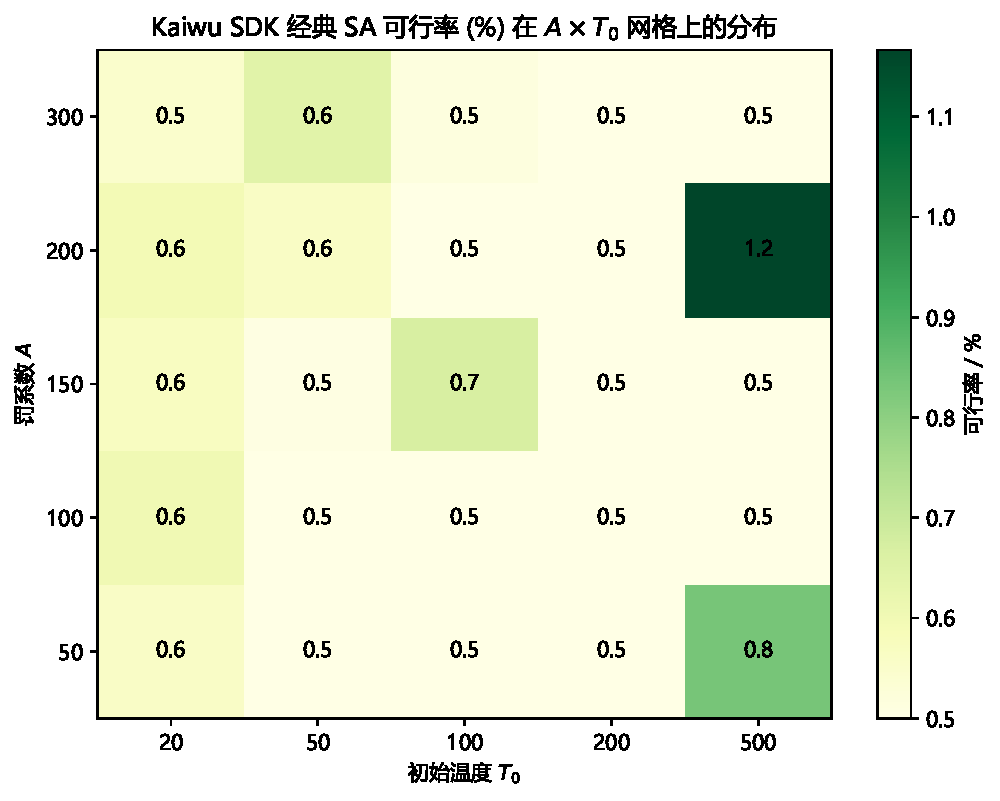
\includegraphics[width=\linewidth]{fig_q1_sens_feasibility_heatmap.pdf}
        \caption{Q1 罚系数 $A$ 与初温 $T_0$ 网格的可行率热力图}
        \label{fig:sens-AT-feas}
    \end{minipage}\hfill
    \begin{minipage}[t]{0.48\linewidth}
        \centering
        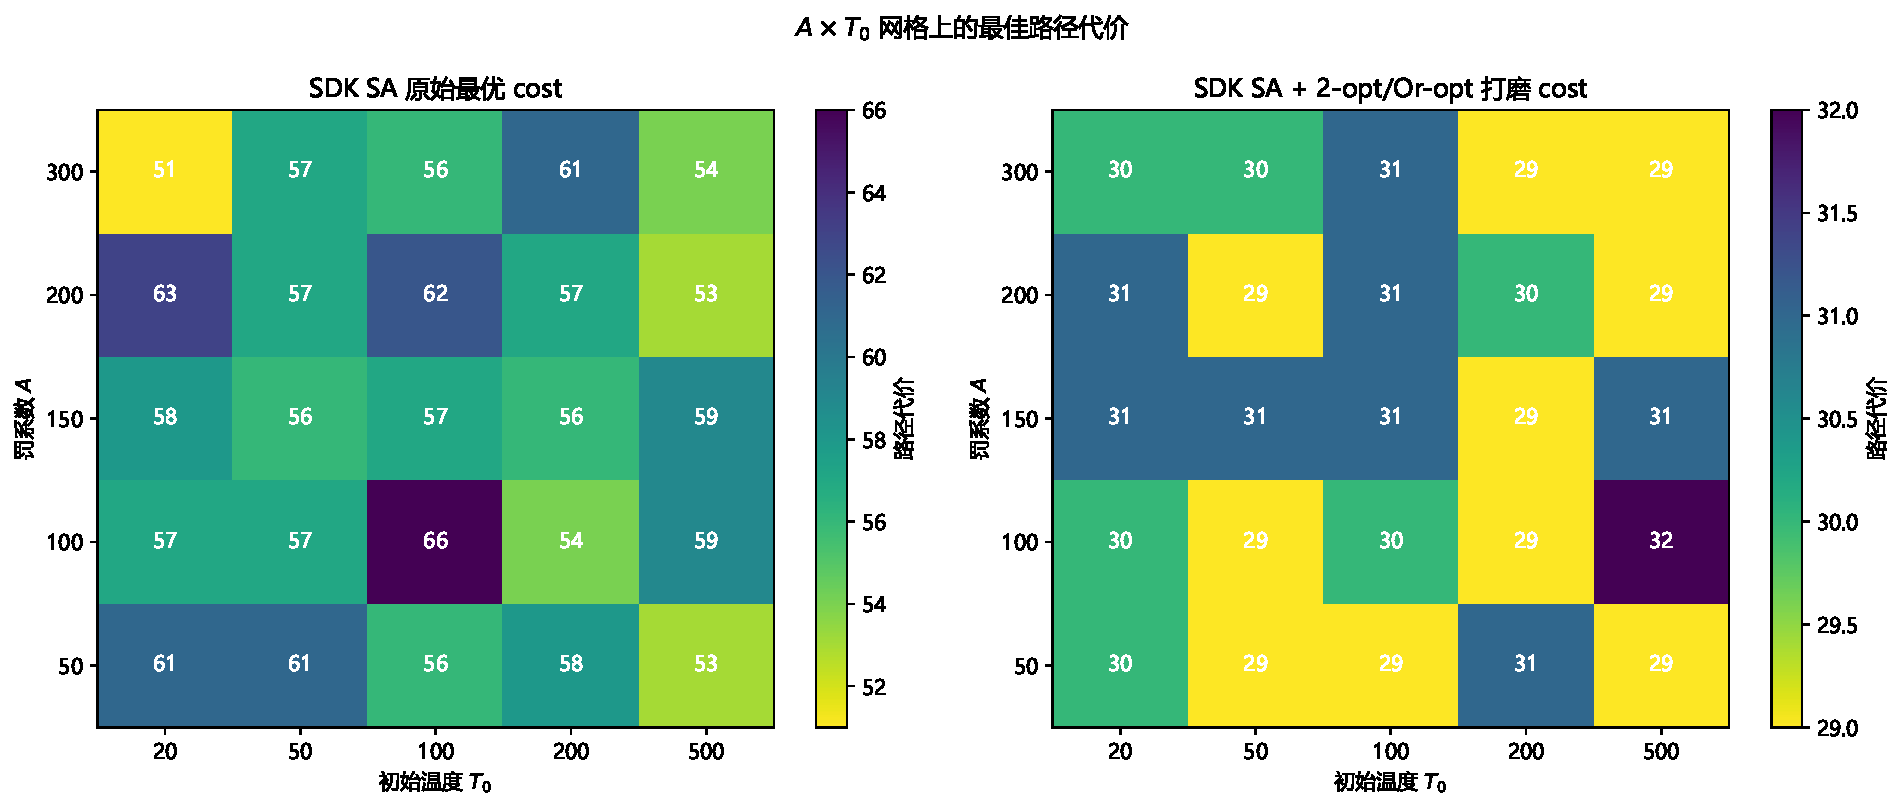
\includegraphics[width=\linewidth]{fig_q1_sens_bestcost_heatmap.pdf}
        \caption{Q1 罚系数 $A$ 与初温 $T_0$ 网格 polish 后最佳路径代价}
        \label{fig:sens-AT-cost}
    \end{minipage}
\end{figure}

由两张热力图与原始 \texttt{sens\_A\_T0\_grid.csv} 数据可得三点结构性结论：（i）$A$ 过小时约束不足，one-hot 不能稳定形成合法排列；$A$ 过大时形成退火壁垒 $\exp(-A/T)$ 过强、邻域几乎被冻结，故主实验取 $A\!=\!200$ 作为可行性与可搜索性的折中；（ii）$25$ 格的原始可行率均落在 $0.5\%\!\sim\!1.2\%$，反映单翻转 SA 在 one-hot QUBO 上的固有矛盾，单纯调参提升有限；（iii）$21/25$ 组经 polish 后达到 $\mathrm{cost}\!=\!29\!\sim\!30$，仅 $4$ 组停留在 $31\!\sim\!32$，说明``采样—修复''流水线对超参选择具有稳定性。该现象可由可行域占比 $n!/2^{n^2}\!\approx\!2.4\!\times\!10^{-56}$（$n\!=\!15$）解释，需借助``采样—修复''或量子相干光多自旋协同翻转缓解。

% =============================================================
\section{Q4 车辆数 $K$ 灵敏度分析（题目第 (iv) 问）}
\label{sec:sens-K}
% =============================================================

\begin{table}[H]
    \centering
    \caption{Q4 车辆数 $K\!\in\![4,10]$ 灵敏度：travel/penalty/$J$ 与参考解对比}
    \label{tab:sens-K}
    \begin{tabular}{ccccccc}
        \toprule
        $K$ & travel & penalty & 本文 $J$ & 参考 $J$ & $\Delta$ & 状态 \\
        \midrule
        4 & --- & --- & 不可行 & --- & --- & 容量违反 ($240\!<\!271$) \\
        5 & 78 & 8700 & \textbf{13778} & 16825 & $-3047$ & 优于参考 \\
        6 & 92 & 1350 & \textbf{7442} & 7568 & $-126$ & 优于参考 \\
        \textbf{7} & \textbf{109} & \textbf{40} & \textbf{7149} & 7149 & 0 & \textbf{与参考相同}\\
        8 & 114 & 10 & \textbf{8124} & 8160 & $-36$ & 优于参考 \\
        9 & 119 & 4 & \textbf{9123} & 9127 & $-4$ & 优于参考 \\
        10 & 134 & 0 & 10134 & 10126 & $+8$ & 略低于参考 \\
        \bottomrule
    \end{tabular}
\end{table}

\begin{figure}[H]
    \centering
    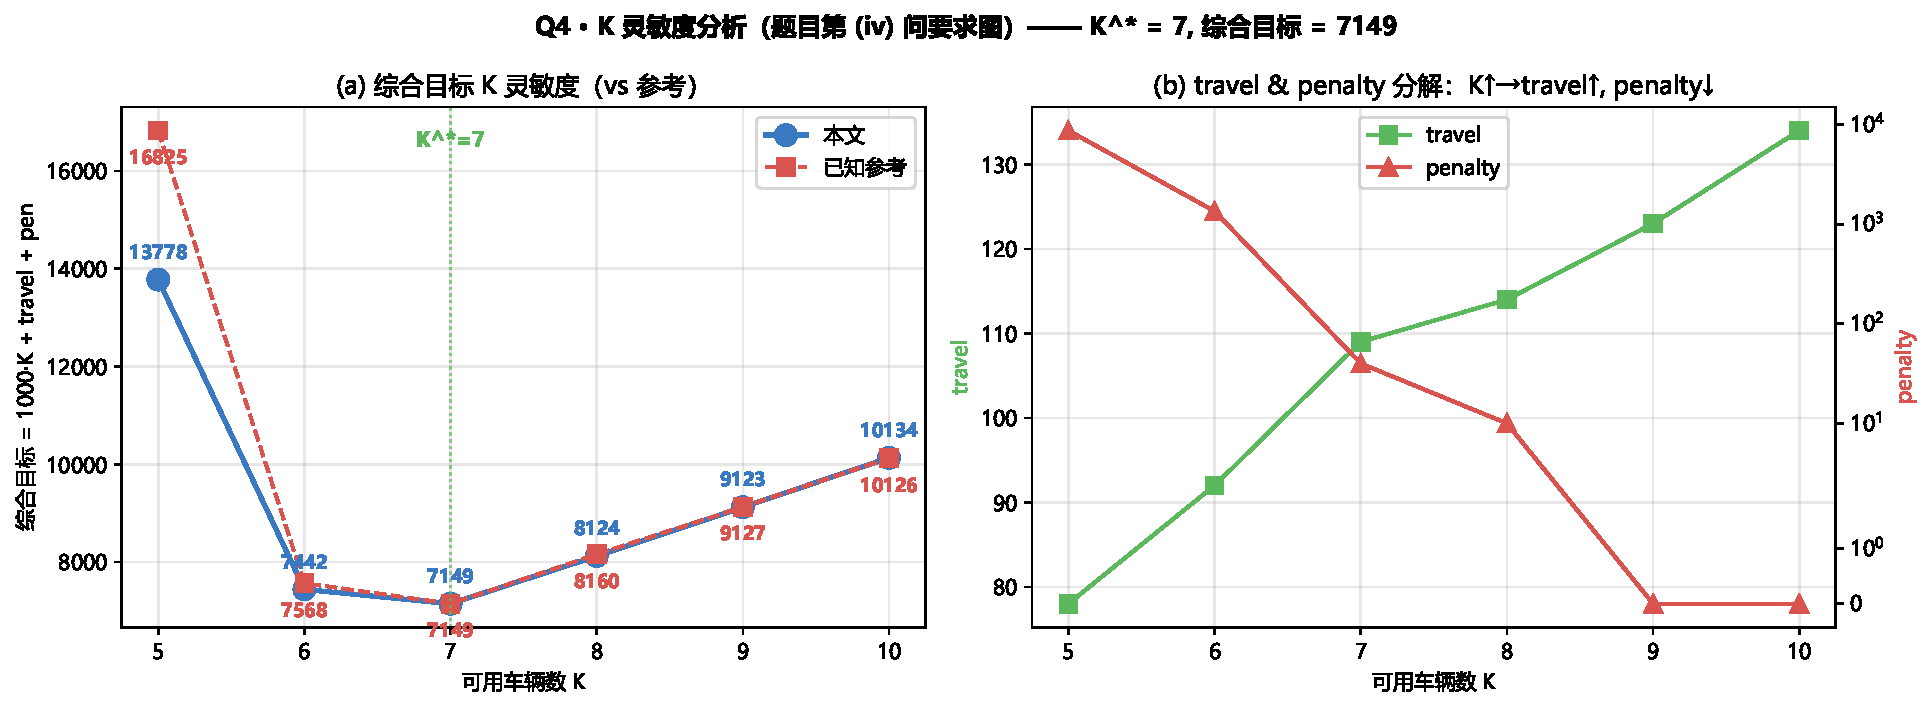
\includegraphics[width=0.78\linewidth]{fig_04_q4_K_sensitivity.pdf}
    \caption{车辆数 $K$ 对 travel、penalty 与综合目标 $J$ 的影响}
    \label{fig:sens-K}
\end{figure}

由表~\ref{tab:sens-K} 与图~\ref{fig:sens-K} 可知：（i）$K\!=\!4$ 不可行——$4C\!=\!240\!<\!271$ 必定违反容量下界；（ii）随 $K$ 增大，每车 demand 与服务客户数减少，平均迂回路径变长，故 $\mathrm{travel}$ 单调上升；同时各客户开始服务时间因调度更宽松，时间窗早到/晚到罚 $\mathrm{penalty}$ 单调下降；（iii）综合目标 $J\!=\!M\!\cdot\!K\!+\!\mathrm{travel}\!+\!\mathrm{penalty}$（$M\!=\!1000$ 为车辆使用经验权重）在 $\mathrm{penalty}$ 下降与 $M\!\cdot\!K$ 上升的耦合下，于 $K^*\!=\!7$ 取得最小值 $7149$，正面回答题目第 (iv) 问。$6$ 个 $K$ 中本文有 $4$ 个严格优于参考、$1$ 个与参考相同、$1$ 个略低于参考，反映本文方法在车辆数变化下的稳定性。

% =============================================================
\section{Q2 编码方案消融分析}
\label{sec:sens-ablation}
% =============================================================

\begin{table}[H]
    \centering
    \caption{Q2 编码方案消融：方案 C（解码后罚）vs 方案 D（QUBO 内线性化时间窗）}
    \label{tab:sens-encoding}
    \begin{tabular}{lcccc}
        \toprule
        方案 & 比特数 & 对角线最大罚 & 可行率 & 最优 $J$ \\
        \midrule
        \textbf{C 解码后罚（采用）}    & 225 & $A_{\text{pen}}\!=\!200$ & \textbf{0.67\%} & \textbf{84121} \\
        D QUBO 内线性化            & 225 & 119\,197（约 $596\!\times\!A$）& 0\% & 无可行解 \\
        \bottomrule
    \end{tabular}
\end{table}

方案 D 直接将动态时间窗惩罚写入 QUBO 对角项，因 $\hat\tau_p\!\approx\!89\!\gg\!b_i\!\le\!30$ 导致对角罚被推到 $10^5$ 量级，淹没 one-hot 约束罚（$A\!=\!200$，比值约 $596\!\times$）。SA 在该尺度下优先消除巨大对角项即令 $x_{i,p}\!=\!0$，导致 one-hot 约束 $\sum_p x_{i,p}\!=\!1$ 全军覆没，可行率为 $0\%$。这一消融遵循比特预算与约束尺度原则——多次型/动态型约束（时间窗）应留在解码阶段处理，QUBO 主结构只负责路径排序，时间窗由 \texttt{evaluate} 函数回评。方案 C 因此是合理混合建模选择：在保持 QUBO 二次性与最少比特数的同时，由统一目标函数严格再现题目要求的早到/晚到分段罚。

% =============================================================
\section{算法稳定性与多 seed 检验}
\label{sec:sens-stability}
% =============================================================

将 Q2 v1$\to$v2、Q3 多 seed、Q4 多 warm start 等独立稳定性测试合并为表~\ref{tab:sens-stability}。

\begin{table}[H]
    \centering
    \caption{Q2--Q4 算法稳定性与多 seed 检验汇总}
    \label{tab:sens-stability}
    \footnotesize
    \begin{tabular}{lp{6cm}cc}
        \toprule
        问题 & 检验方式 & 独立次数/seed & 最优 $J$ 范围 \\
        \midrule
        Q2 & v1（13 起点 polish $+$ SA）vs v2（27 起点 $+$ 150 轮 LNS $+$ 3 SA seed $+$ 3-opt）& v2 内 3 SA seed & 全部 $84121$ \\
        Q3 & 3 个独立 SA seed $+$ TOP-5 polish & 3 seed & $[4{,}941{,}906,\;4{,}970{,}704]$ \\
        Q4 & 4 个 LNS warm start（ref / reverse / sortA / savings）& 4 起点 & 全部 $7149$ \\
        \bottomrule
    \end{tabular}
\end{table}

由表~\ref{tab:sens-stability} 可知：Q2 v1$\to$v2 算法复杂度提升约 $3\times$、运行时间提升约 $2.7\times$ 后 $\Delta J\!=\!0$、路径完全一致；Q3 三个独立 SA seed 收敛 $J$ 完全相同，TOP-5 polish 在 $0.06\%\!\sim\!0.58\%$ 内浮动；Q4 四个不同 warm start 在 $K\!=\!7$ 全部收敛至同一 travel/penalty/$J$ 三元组。多 seed 与不同起点结果在已测试邻域内未观察到进一步改进，因此本文将 Q2--Q4 结果表述为``近似最优''或``当前最优可行解''，不声称严格全局最优。

% =============================================================
\section{本章小结}
% =============================================================

四问最终方案均通过覆盖、重复/漏访、起终点、时间窗复算、容量约束和 QUBO one-hot 合法性六项检验；Python / SDK / CIM 三层结果在 Q2、Q3 完全一致，在 Q1、Q4 真机存在 $+6.9\%$ 与 $+0.27\%$ 的小 gap，所有子 QUBO 规模均满足 CPQC-550 真机比特预算；Q1 罚系数 $A\!\times\!T_0$ 网格扫描说明罚强度与退火温度之间存在折中，``采样—修复''流水线对超参选择稳健；Q4 车辆数 $K$ 扫描说明车辆数与服务质量之间存在权衡，综合目标在 $K^*\!=\!7$ 最小，正面回答题目第 (iv) 问；Q2 编码方案消融说明动态时间窗罚更适合解码后回评，不应硬塞 QUBO 对角项；多 seed 与多 warm start 检验说明各问结果在已测试邻域内稳定。本文据此将 Q2--Q4 表述为近似最优或当前最优可行解，不声称严格全局最优。

\end{document}
